%##############################################################
\section{Fast Automatic Gain Control for SDR Systems}
\label{wurc_agc}

In radio communications, receivers must tolerate a wide range of input power levels in order to accommodate both near and distant transmitters; this effect is aggravated in large-scale UHF systems.
For example, the free-space path loss for a 400~MHz system operating over 10~km is $(\frac{4\pi d}{\lambda})^{2} = 104.5$~dB. This can present serious problems to the \ac{ADC} subsystem of a software-defined radio receiver if it must be capable of decoding signals from both nearby transmitters and those at a distance.

Intuitively, imagine a noisy room where one guest is yelling through a megaphone into your ear while another is whispering quietly in a corner; it would be difficult to understand what they were saying in either case.

Technically, the cause of distortion in a strong signal comes from the inability of an \ac{ADC} to distinguish between input voltage levels above and below its maximum and minimum codeword values.
This results in a phenomenon called \textit{clipping} where the analog signal is limited in its digital representation to the upper and lower bounds of the \ac{ADC} codeword, thus destroying information in the signal.
When the \ac{ADC} encounters this condition, we call it \textit{saturated}.

For a weak signal, distortion is generated when variation in the input signal is smaller than the minimum resolution of the \ac{ADC} or it becomes indistinguishable from systemic noise in the receiver.
Under these conditions, we say the signal is below the resolution of the \ac{ADC} or \textit{under-resolved}.

In addition, the amount of \ac{ADC} quantization error is proportional to the relative size of the quantization steps and the power of the signal of interest \cite{middleton2007agc}.
Thus, there is incentive to ensure that the power of the input signal is as large as possible without saturating the \ac{ADC}.

\ac{AGC} systems attempt to estimate the power input to a radio receiver and adjust the analog gains of that receiver in order to ensure that the \ac{ADC} input signal power falls within an optimal window and is not saturated while ensuring sufficient resolution available for the signal of interest.

\begin{figure}[t] % Idealized AGC block diagram
\centering
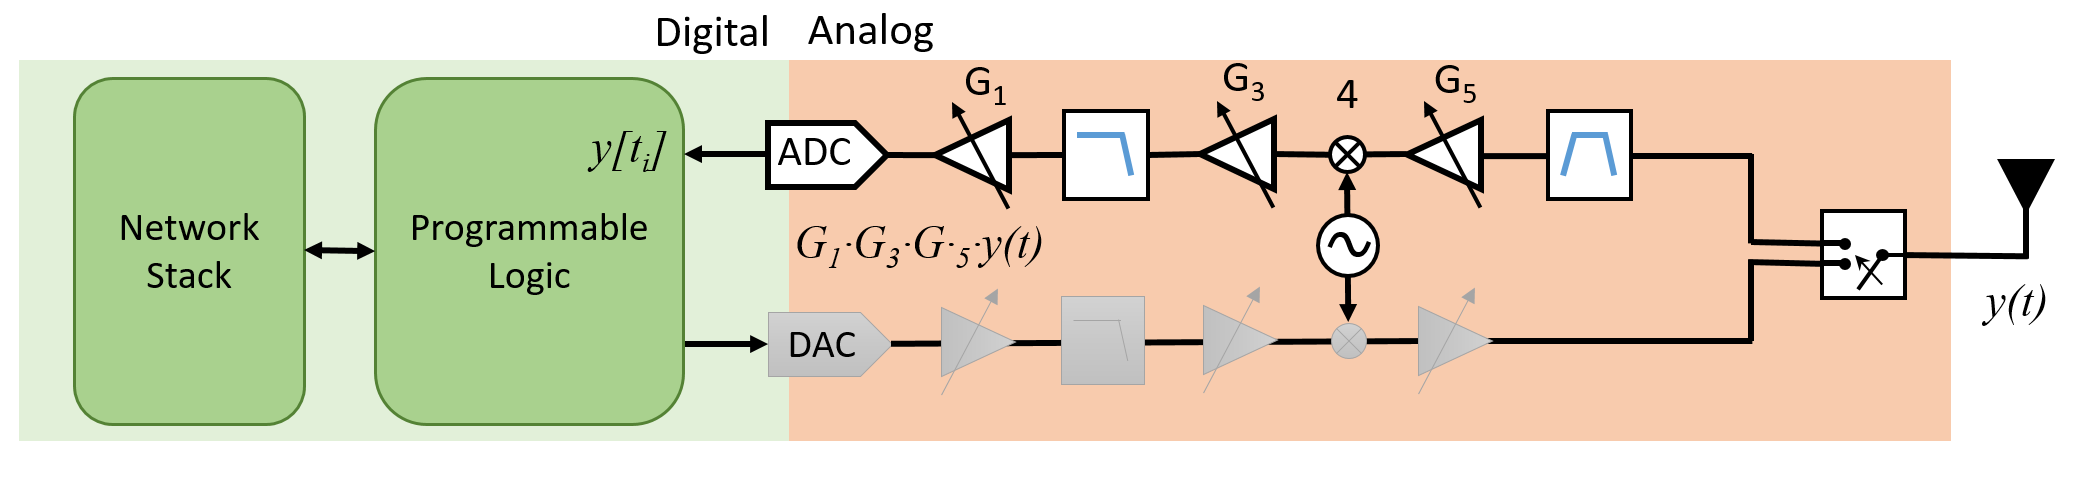
\includegraphics[width=1\linewidth]{./figs/agc/agc_rx_diagram}
\caption{Block diagram of the software-defined radio receive chain.}
\label{fig_sdr_ideal_rx}
\end{figure}

Figure~\ref{fig_sdr_ideal_rx} shows our block diagram of a generic software-defined radio system's receive chain with three programmable gain blocks: pre-mixer $G_5$, post-mixer $G_3$, and post-filtering $G_1$ that together control the input gain to the \ac{ADC}.
Under ideal conditions, when the input signal $y(t)$  is perfectly band-limited and all components are linear, the signal present at the \ac{ADC} input, $G_1\cdot G_3\cdot G_5\cdot y(t)$, will be converted to a digitally sampled signal, $y[t_i]$, that contains the full information present in the input signal $y(t)$.

In this section, we present the design, hardware implementation, and over-the-air validation of a new \emph{analog} \ac{AGC} subsystem designed for the \ac{WURC}.
This \ac{AGC} subsystem is novel in that it does not require the assistance of an external analog power estimation block and can therefore be implemented on any \ac{SDR}, yet it can still converge rapidly within the strict time constraints of common random-access communications standards such as IEEE 802.11 \cite{std11_2012}.
This differs from \ac{AGC} systems implemented on other \ac{SDR} platforms such as WARP \cite{middleton2007agc, warp} or SORA \cite{sora} that respectively utilize other analog circuitry or have a slow update loop limited by software processing times.

This novel architecture enables the implementation of critical \ac{AGC} functionality in systems that may be limited in analog hardware yet have sufficient real-time digital resources to implement our solution.

%#######################################
\subsection{AGC Design Specification}

The design goal of our \ac{AGC} system is to adjust the receive gains in our system such that any incoming packet with \ac{RMS} power between $[-103.6, -15.1]$~dBm at the input antenna port will have \ac{RMS} power between $[-42.6, -15.1]$~dBm when it reaches the \ac{ADC} as shown in Figure~\ref{fig_sdr_ideal_rx}.
Convergence to stable recieve gain values should be complete within $5.6~\mu s$ after reception of a inbound data packet.
We consider this ``fast'' \ac{AGC} since the gain is being dynamically adjusted on a symbol-level timescale ($\mu s$) rather than a packet timescale ($ms$).
In fact, we will see how many architectural decisions are guided by this relatively short timeframe.

These particular values are selected based on the parameters of the \ac{WURC} transceiver hardware \cite{lime2012lms6002d} and the expected characteristics of our signal waveform \cite{perahia2013next}; however the following design procedure can generally be applied to any \ac{SDR} system.

%=========================
\subsubsection{ADC Dynamic Range}
\label{sec_adc_dyn_range}

\begin{figure}[h] % AGC Design Diagram
\centering
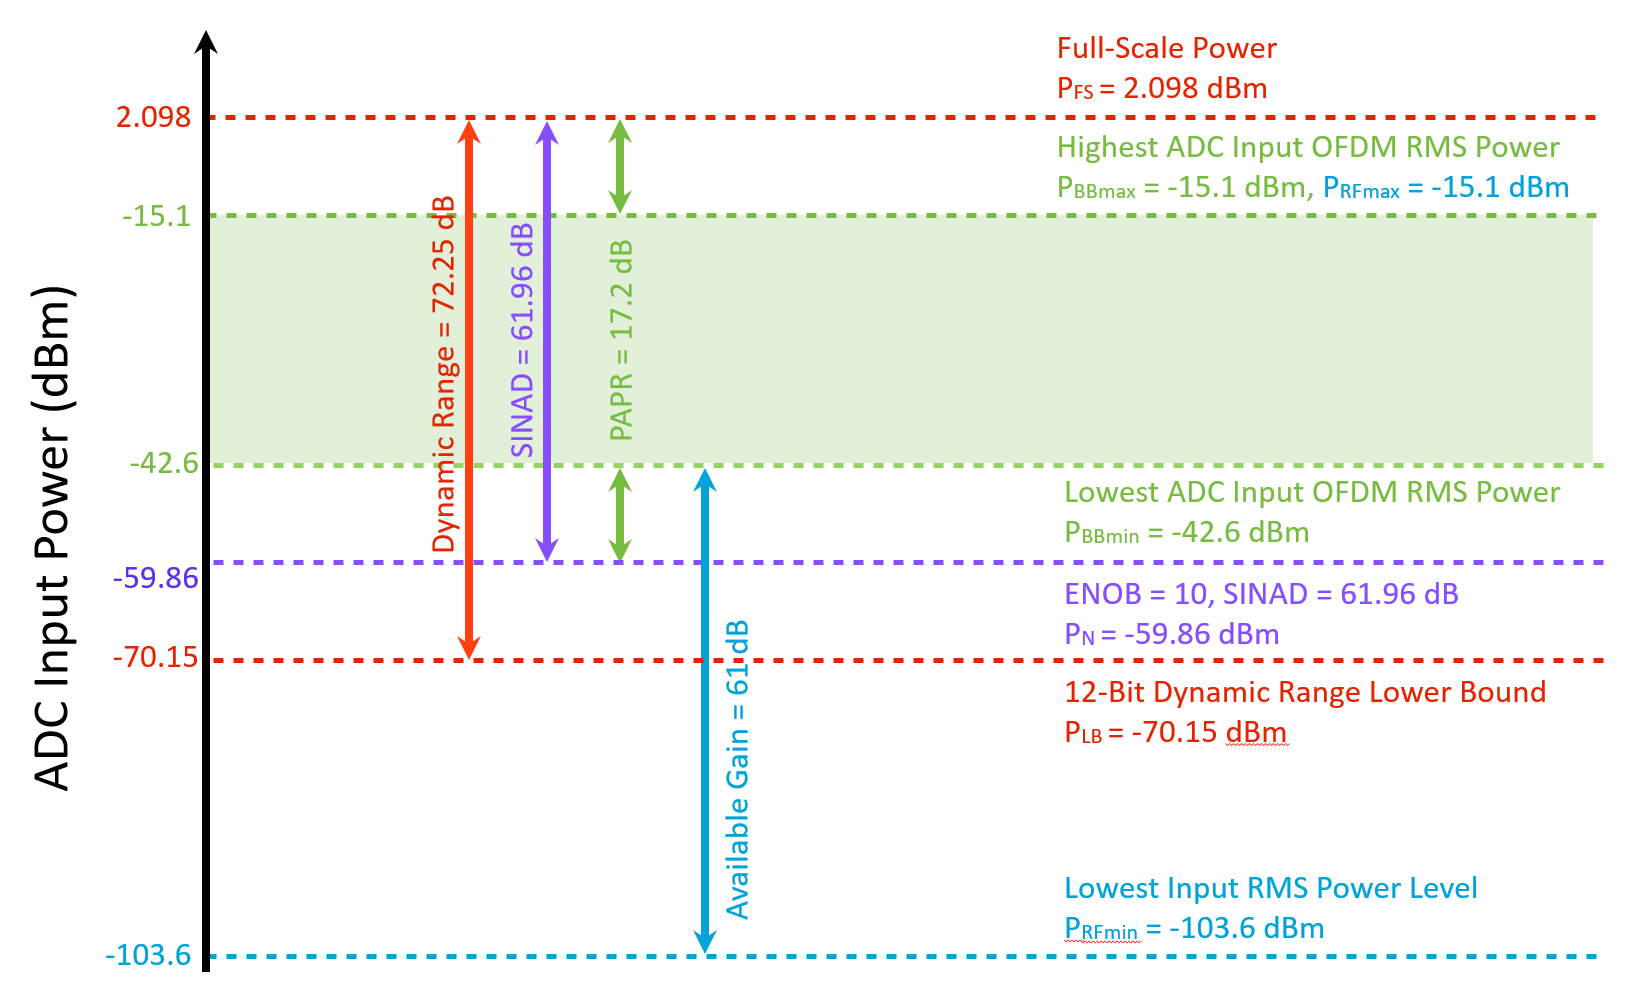
\includegraphics[width=1\linewidth]{./figs/agc/agc_dynamic_range}
\caption{Illustration of AGC resolution, system available gain, and signal dynamic range for the LMS6002D \cite{lime2012lms6002d}.}
\label{fig_agc_dynamic_range}
\end{figure}

\ac{ADC} components are characterized by their \ac{ENOB}, or the number of bits available for the digitization of signals after accounting for the systemic noise generated by the \ac{ADC} circuitry, and their \ac{FSR}, or the minimum and maximum voltage values that can be encoded by the \ac{ADC}.
These two values provide the lower and upper bounds, respectively, of the \ac{ADC} power resolution \cite{adi2008sinad}.
Since the voltage of an \ac{ADC} is measured across a static resistive load, voltage level bounds translate directly into power level bounds.

Formally, \ac{FSR} is defined as:
\begin{equation} \label{eq_fsp}
\text{FSR} := P_{FS} = \frac{V_{MAX}^2}{R_{ADC}} = \frac{(1.8)^2~\text{V}^2}{2000~\Omega} = 2.095~\text{dBm},
\end{equation}
where $V_{MAX}$ is the voltage of the maximum ADC codeword and $R_{ADC}$ is the value of the ADC load resistor in Ohms \cite{lime2012lms6002d}.

\ac{SINAD} is defined as the ratio of the desired signal to noise and distortion from all sources excluding the power of the DC spectral component \cite{adi2008sinad}.
As an empirically determined specification, it captures the practical dynamic range of an ADC by incorporating ADC non-linearities and distortions and indicating the level at which a desired signal would become indistinguishable from interfering signals.
When the input signal is a full-scale sinusoid, it is related to the \ac{ENOB} according to the following relationship that follows from the definition of an ideal ADC \cite{rohde2011enob}:

\begin{equation} \label{eq_enob}
\text{SINAD} := \text{ENOB} \cdot 6.02 - 1.76~\text{dB}.
\end{equation}

The \ac{SINAD} is plotted in Figure~\ref{fig_agc_dynamic_range}, where it defines the operational range of the \ac{ADC}.

%===========================
\subsubsection{Peak-to-Average Power Ratio}
\label{sec_agc_papr}

The 802.11ac and 802.11af standards define a high throughput mode that utilizes \ac{OFDM} waveforms for physical-layer communication \cite{perahia2013next, flores2013ieee80211af}.
Due to the statistically independent nature of the symbols transmitted on each subcarrier, the overall time-domain signal of a wideband \ac{OFDM} waveform with many subcarriers may be modeled as a zero-mean random Gaussian process \cite{proakis1995digital}.
Modeled thus, the ratio of the highest power time-domain sample to the mean time-domain sample grows with the variance of the aggregate Gaussian process, or grows with $\sqrt{K}$, where $K$ is the number of subcarriers.

When a signal is represented as a series of time-domain complex values, $s[t_i]\in \mathbb{C}$, indexed by time $t_i$, we can define the \ac{PAPR} \cite{bauml1996reducing}: 
\begin{equation}
\text{PAPR} := 10 \cdot\log_{10}(\frac{\max_{i}(|s[t_i]|^2)}{\mathbb{E}\{|s[t_i]|^2\}}).
\end{equation}

For 802.11af, a 20~MHz VHT frame contains 52 subcarriers, resulting in a worst-case \ac{PAPR} of approximately 17.2~dB.
In order to guarantee that reception of this signal can take place without clipping at the ADC, the input power at the ADC should be less than 17.2~dB below the ADC's \ac{FSR}.
Similarly, in order to guarantee that time-domain samples are not under-resolved, the input power to the ADC should be more than 17.2~dB above the ADC's effective noise floor (FSR - SINAD).
These two additional \ac{PAPR} margins (green) are illustrated in Figure~\ref{fig_agc_dynamic_range} to yield the target operational range of the ADC (shaded green region).

Other literature has focused on how the \ac{PAPR} of signals may be reduced with digital pre-processing steps \cite{bauml1996reducing}, however we assume these techniques will not be applied to the standard 802.11af waveform.
If \ac{PAPR} mitigation techniques, also know as \emph{crest-factor reduction}, are utilized, this will simply decrease the required \ac{PAPR} margin in our design accordingly.


%===========================
\subsubsection{AGC Timing Constraints}
\label{sec_agc_timing}

	A necessary condition for generic fast analog gain control to be feasible is that the digital logic must be able to react to and effect changes in the analog gain blocks within the deadline allowed for \ac{AGC} operations.
	This becomes particularly important in random-access systems like 802.11 since the receiver generally doesn't have information about the transmitter until after its signal is already being processed and therefore must rapidly adapt reception parameters in order to detect and decode the received packet accurately.

	Perhaps the most challenging requirement of the \ac{WURC} AGC system design is that of meeting the strict 802.11af/ac frame timing.
	In this section, we analyze the timing constraints of our particular \ac{SDR} system and what this means for other system implementations of our fast \ac{AGC} system.

\textbf{Frame Preamble Timing.} The \ac{PLCP} component of the 802.11 standard defines a common preamble for packet transmissions that enables receiving devices to synchronize to the transmitted waveform \cite{perahia2013next, 80211ac} and simplifies interaction with higher layer of the network stack.
	Displayed logically in Figure~\ref{fig_agc_80211_plcp}, the \ac{PLCP} consists of two training fields of $8~\mu s$ for receiver synchronization and a \emph{SIGNAL} field of $4~\mu s$ containing rate and data length information for the rest of the packet or \ac{PPDU}.

\begin{figure}[h] % Idealized AGC block diagram
\centering
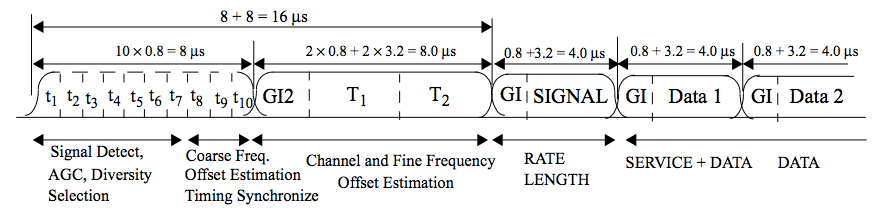
\includegraphics[width=1\linewidth]{./figs/agc/agc_80211_plcp_format}
\caption{IEEE 802.11-2012, \S18.3.3 \ac{PLCP} preamble format and timing \cite{std11_2012}}
\label{fig_agc_80211_plcp}
\end{figure}


	While precise receiver operation is not specified in the 802.11 standard, generally the first 7 sub-fields of the short training field, L-STF, are reserved for packet detection, gain control, and antenna diversity selection.
	The fields are labeled $t_1$ through $t_7$ in Figure~\ref{fig_agc_80211_plcp}.
	The remaining 3 fields of the L-STF and the long training fields, L-LTF, are reserved for timing recovery, channel estimation, and transmitter frequency offset calculation \cite{perahia2013next}.

	In this particular \ac{SDR} realization, that means that incoming packets must be detected and gains must be dynamically set within $5.6~\mu s$ in order to meet the timing constraints given in the 802.11 standard.
	For 40~MHz \ac{ADC} sampling rates, that's less than 224 samples since the \ac{AGC} system must perform signal processing; at 20~MHz sampling rate, the system must react with less than 112 samples of data.

\textbf{Serial Interface Timing.} The LMS6002D transceiver containing the receive variable-gain amplifiers is controlled by a \ac{SPI} controller accessing an 8-bit command register space \cite{lime2012lms6002d}.
	Each write command consists of an 8-bit instruction concatenated with an 8-bit data payload.
At a maximum interface speed of 50~MHz, it takes $0.32~\mu s$ to complete each \ac{SPI} transaction.
	Gain settings for the LMS6002D transceiver require \ac{SPI} transactions to three separate registers; however, we observe that one register controls the first-stage \ac{LNA}, which should always be left active for noise performance and should therefore not be adjusted by the \ac{AGC} system.
	Since it take approximately 100~$ns$ for the receive gain stages to settle once programmed, we can expect at least 0.74~$\mu s$ of delay for each change in receive gain to be implemented, or around 14\% of the total timing budget allowed.

	In general, our design for an analog \ac{AGC} system must be able to set receive gains several times within the time budget allocated since it can not rely on saturated digital observations to estimate the input power to the \ac{ADC}.
	Other commercial \ac{SDR} platforms (\emph{e.g.} based on AD9363, ADRV9009, or LMS7002M transceivers \cite{adi2016ad9363, adi2018adrv9009, lime2018lms7002M}) operate on similar timescales with respect to digital control interfaces, making our design feasible across a wide range of SDR platforms.


%##############################################################
\subsection{Alternative AGC Architectures}
\label{sec_agc_related}

In this section, we present a detailed comparison of our approach with alternative \ac{AGC} systems used in other commercial \ac{SDR} systems.

\subsubsection{Digital Gain Control}
\label{sec_agc_dig_alt}

\begin{figure}[h] % AGC Design Diagram
\centering
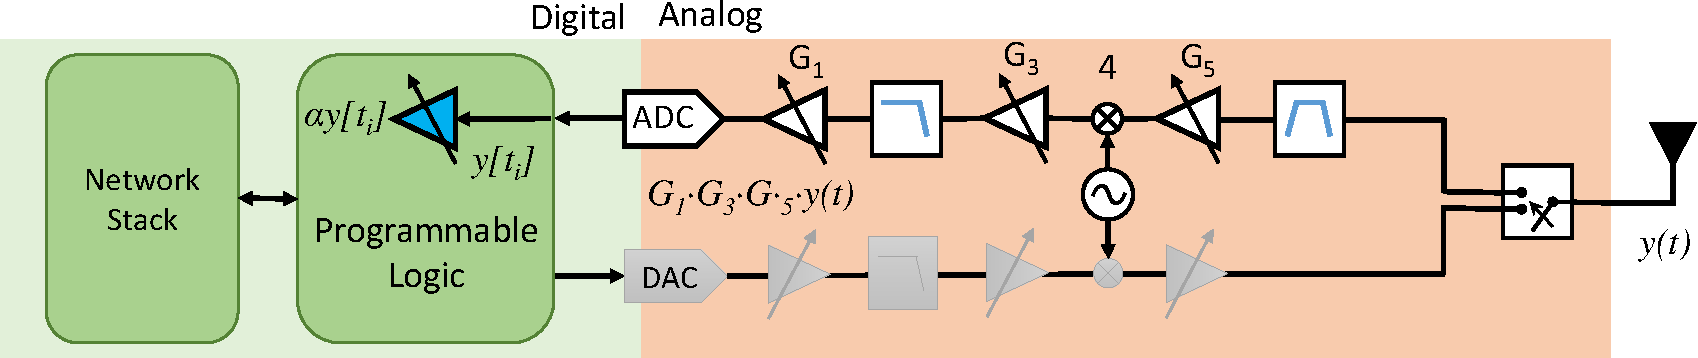
\includegraphics[width=0.9\linewidth]{./figs/agc/agc_digital_diagrams}
\caption{Diagram of digital gain control circuitry (blue).}
\label{fig_dig_agc_diagram}
\end{figure}

	When \ac{DSP} processing blocks are designed with fixed point precision, it is sometimes critical to ensure that the input \emph{digital} signals do not exceed certain minimum or magnitude bounds in order to avoid numerical precision errors or overflow.
	For that reason, \emph{digital} automatic gain control is often implemented in radio systems in order to ensure the integrity of downstream fixed precision processing blocks \cite{lee2006agc}.
	In Figure~\ref{fig_dig_agc_diagram}, we show that these subsystems are generally implemented in the programmable logic of the \ac{SDR} with a digital gain block, providing a scalar gain of $\alpha$ multiplied with the digital IQ sample stream before being further processed. 
	
	However, once the baseband analog signal has been sampled at the \ac{ADC}, any chance to avoid under-resolved or clipped analog signals is lost, thus its utility is somewhat limited.
	Therefore, our approach of using digital feedback to control analog gain rather than digital gain can be used to meet both the requirement of reliable signal magnitude for fixed-precision \ac{DSP} blocks as well as analog signal power within the operational range of the \ac{ADC}.


\subsubsection{Analog Input Power Estimation}
\label{sec_agc_analog_alt}

\begin{figure}[h] % AGC Design Diagram
\centering
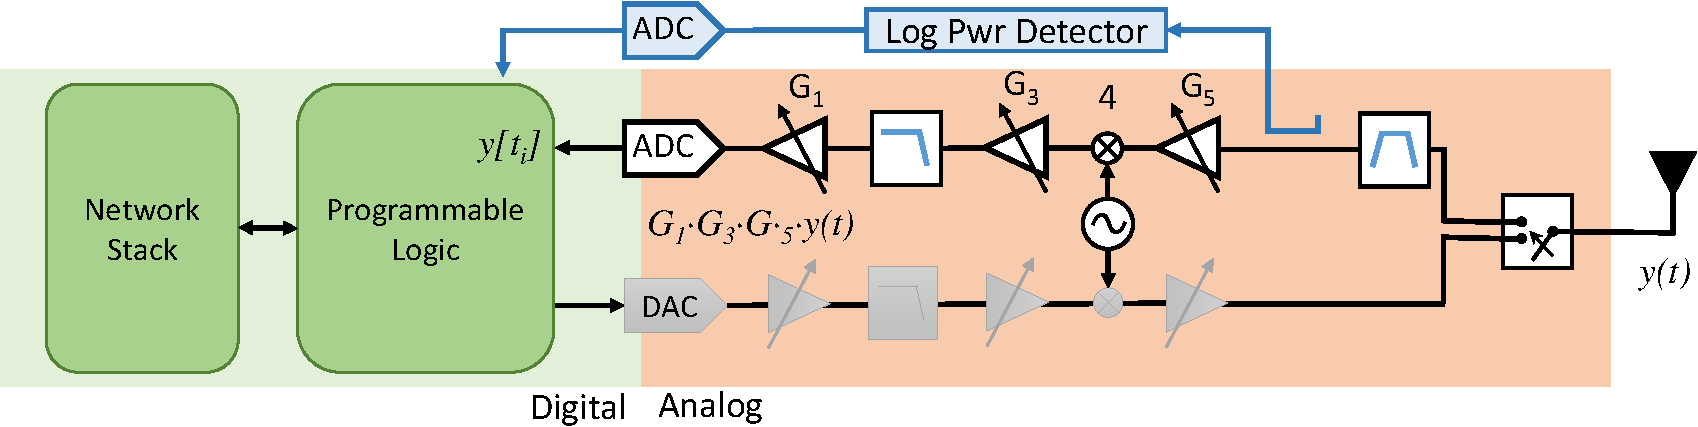
\includegraphics[width=0.9\linewidth]{./figs/agc/agc_diagrams_analog}
\caption{Diagram of analog power detection circuitry (blue).}
\label{fig_pwr_detection_diagram}
\end{figure}

	The most commonly used alternative architecture for analog gain control for \acp{SDR} is to directly estimate the input power to the \ac{SDR} at the input antenna port using a power coupler,\footnote{Alternatively, this estimation can take place at any point along the receive chain, provided gains between the measurement point and the input to the \ac{ADC} are known.} log power detection circuitry, and an auxiliary \ac{ADC} to convert the sensed analog power to a digital representation Figure~\ref{fig_pwr_detection_diagram} (blue).

	When designing \ac{WURC}, we first implemented analog power detection in our first development PCB prototype.
In Figure~\ref{fig_pwr_detection_proto}, we show a prototype analog gain control circuit utilizing a Maxim MAX2015 log-power detector and the built-in \ac{ADC} within the Stellaris microcontroller (bottom right PCB).
This same architecture was used to develop the Lime Microsystems LMS6002D control library \cite{guerra2013lms6002d}.

\begin{figure}[ht] % AGC Design Diagram
\centering
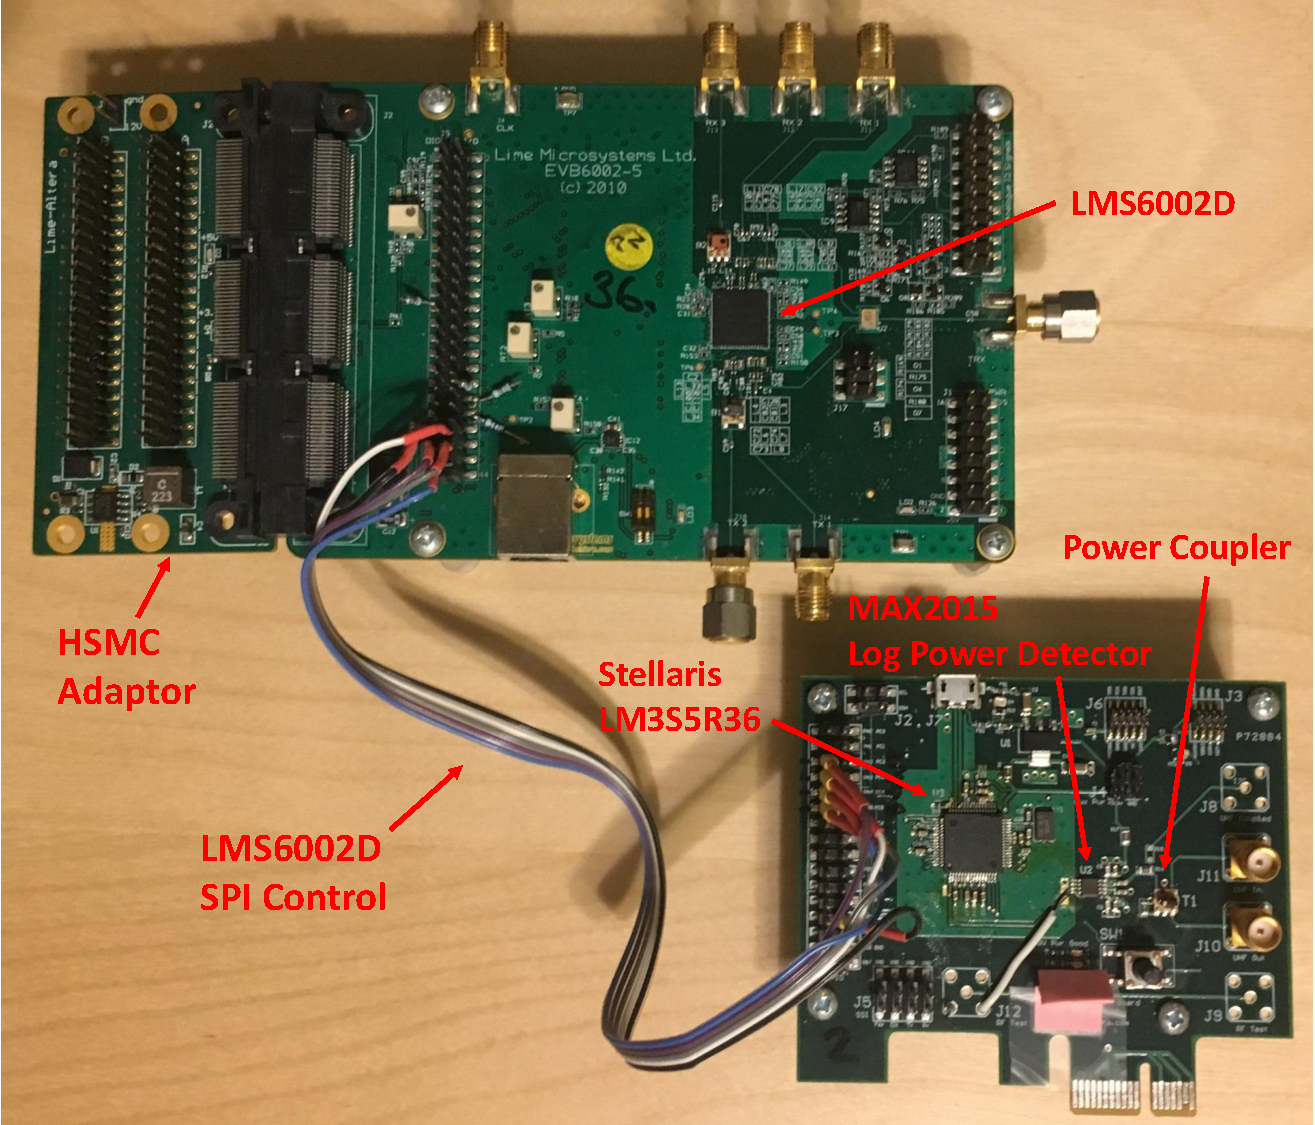
\includegraphics[width=0.9\linewidth]{./figs/agc/agc_dev_board}
\caption{Prototype analog log-power detector and LMS6002M development PCB.}
\label{fig_pwr_detection_proto}
\end{figure}

Three challenges were encountered:
	First, the extra analog power estimation components require additional cost and impose constraints on circuit layout and signal integrity.
	Second, and more subtlety, the division of gain control logic between multiple components requires synchronization and overhead that begins to eat into the \ac{AGC} timing budget.
For example, in our implementation, the Stellaris LM3S5R36 required a significant delay to estimate input power, make receive gain and packet detection decisions, and issue gain setting commands to the LMS6002D transceiver.
	Third, the MAX2015 has a dynamic detection range between -65 and +5~dBm, whereas we already expect to support packet reception well below -65~dBm.
	An additional RF amplifier could be provisioned to boost the detector input level or the RF coupler could be inserted somehow after various gain stages, however the former approach would add additional system cost and the latter was not possible with our highly-integrated LMS6002M transceiver IC.

	Instead, by eliminating analog power detection circuitry and integrating these functions within the digital \ac{SDR} logic in our proposed design, we reduced the overall cost and complexity of the radio design and provided tighter integration of \ac{DSP} logic and gain control functions to improve reaction speeds.
	
		The most recent generation of \ac{SDR} transceivers are starting to integrate this type of analog power estimation circuitry \cite{adi2018adrv9009}; however, our final design can be implemented in legacy \ac{SDR} devices that don't provision analog circuitry, increasing the number of systems that can benefit from our approach while providing equivalent performance.

%##############################################################
%\subsection{Fast Hybrid Packet Detection}
%\label{sec_pkt_detection}
%
%\rgnote{Packet detection across a wide range on input signal levels is difficult with any one detection technique; thus we design a hybrid detector that uses both energy detection and cyclostationary detection (autocorrelation) to quickly detect an incoming packet reliably and trigger AGC.}
	%
%\begin{figure}[h] % AGC Design Diagram
%\centering
%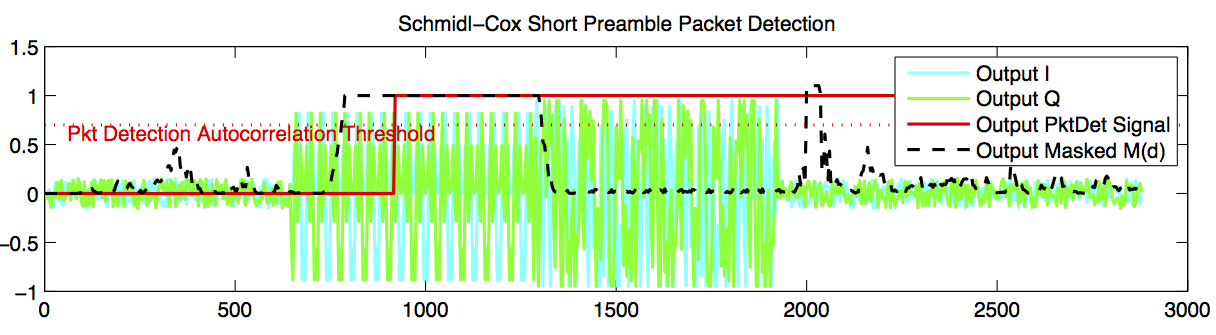
\includegraphics[width=1\linewidth]{./figs/agc/agc_schmidtl_cox_autocorrelation}
%\caption{Example of digital autocorrelation packet detection.}
%\label{fig:agc_autocorr}
%\end{figure}
%
%A key observation is that detecting a saturated  or strong input signal is more reliable and quicker than detecting an under-resolved or weak signal.

%##############################################################
\subsection{Hybrid Packet Detection}
\label{sec_pkt_detection}

	The challenge with implementing \ac{AGC} with only the input of the \ac{ADC} as a reference is that signals that fall outside of the ADC's dynamic range are unreliable.
	Taking the 802.11af standard as a reference, it may not only be difficult to detect the incoming packet when the digital samples are under-resolved or clipped, but any input power estimate will also be inaccurate since the digital samples are not capturing the full power of the incoming signal.

	Our solution is to approach this problem in steps: first, detect that a packet is being received; second, quickly detect and remove saturation with coarse gain steps; third, once saturation has been removed, fine-tune receive gains with a reliable estimate of the \ac{ADC} input power.

	The first step is addressed by utilizing the Schmidl-Cox digital packet and timing detection technique \cite{schmidl1997robust} for sensitivity in parallel with an energy detection block for quick packet detection.
	
\begin{figure}[ht] % Packet Detection Example
\centering
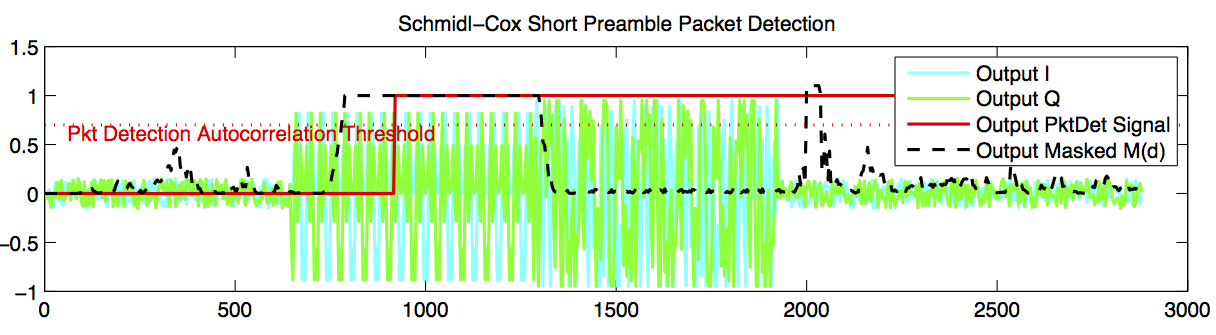
\includegraphics[width=1\linewidth]{./figs/agc/agc_schmidtl_cox_autocorrelation}
\caption{Example of digital autocorrelation packet detection.}
\label{fig_agc_autocorr}
\end{figure}
	
	The Schmidl-Cox detector works by auto-correlating the input signal and normalizing this result by the input power level in order to produce a large detection metric $M(d)$ when a repetitive signal with period equal to the 802.11 short timing sequence period is observed (0.8~$\mu$s, Figure~\ref{fig_agc_80211_plcp}).
	A simulation of digital packet detection using this method is shown in Figure~\ref{fig_agc_autocorr}, where the in-phase (I) and quadrature component (Q) are given in green and cyan, the auto-correlation metric value is shown in black, and the packet detection decision is shown in red (transition from $0 \rightarrow 1$).
	In order to reject false-positive packet detection, the Schmidl-Cox detector waits for the decision metric $M(d)$ to cross a threshold (red dotted line) for a specified period of time.
	
	Both the value of the threshold and the number of samples required to be above that threshold before deciding a packet is detect can be adjusted to tune the probability of a false-positive and missed-detection.
	We show the simulation in Figure~\ref{fig_agc_autocorr} at relatively low \ac{SNR} value in order to demonstrate that the Schmidl-Cox detector is relatively slow to produce a decision even under ideal conditions: by the time the packet detection signal is raised, over half of the 5.6~$\mu$s time budget for \ac{AGC} has been consumed.
	
	In contrast, a simple energy-based detection algorithm can react relatively quickly, during the first 0.8~$\mu$s, however it has fundamental detection limits for low-\ac{SNR} signals in the presence of noise \cite{shellhammer2006performance}.
	Our key observation is that energy detection works well and quickly for high-\ac{SNR} signals, which is when we will need additional time to remove potential \ac{ADC} saturation.
	In contrast, auto-correlation techniques perform well but respond slowly for low-\ac{SNR} signals, where we may expect little to no \ac{ADC} saturation.
	
	In our design, the packet detection is taken as the logical-OR of the detection output of both detectors, resulting in the best-case packet detection performance in both high-SNR and low-SNR regimes.
	The transceiver's idle receive state is initially set to maximum receive gain, ensuring that even weak packets will be detected reliably.

	%\rgnote{it really would be great to have a plot here showing detection probabilities or detection speeds for various detection methods... this could be actual hardware-in-the-loop or simulation, both are relatively easy.}

%##############################################################
\subsection{Coarse Gain Control for Saturation Removal}
\label{sec_coarse_gain}

	Once a packet is detected via energy or auto-correlation detection methods, we then wish to detect and remove \ac{ADC} saturation.
	Lee \emph{et. al.} \cite{lee2006agc} proposed a digital saturation detector aimed at adjusting the \emph{digital} gain level for fixed-precision digital logic in \ac{OFDM} transceivers.
	We utilize this same saturation detection logic in order to instead detect \emph{analog} \ac{ADC} saturation.
	Our implementation is presented in Figure~\ref{fig_agc_sat_block}, where the raw I and Q streams are independently observed for saturation conditions: crossing a magnitude threshold a specific number of times (3) within a window of 16 samples.
	If at any time more than 3 samples are observed above this conservative threshold, the input is declared ``saturated;'' however at least 16 consecutive samples must be observed after reset before the input can be declared ``not saturated.''

\begin{figure}[ht] % AGC Saturation Detection Block Diagram
\centering
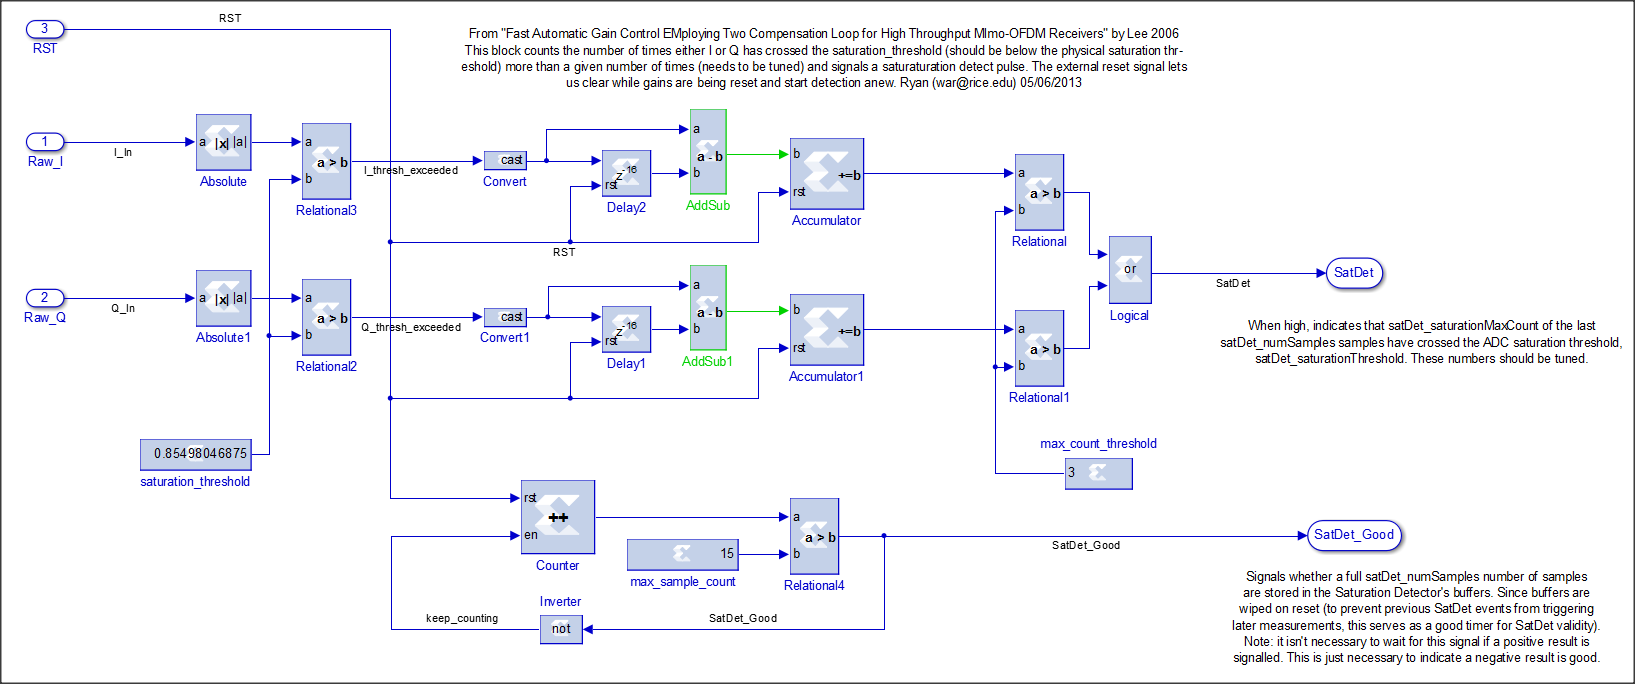
\includegraphics[width=1\linewidth]{./figs/agc/agc_saturation_block_implementation}
\caption{Digital logic block diagram implementation of ADC saturation detection.}
\label{fig_agc_sat_block}
\end{figure}

	Once saturation is detected, the analog receive gain is reduced in large steps to remove it.
	Since the ideal dynamic range of the \ac{ADC} is $[-15.1, -42.6]$ as per our calculations in Section~\ref{sec_adc_dyn_range}, we back off analog receive gains by 27~dB each time that saturation is detected on the \ac{ADC}.
	This results in decision regions as shown in Figure~\ref{fig_agc_coarse_gain}: if the input signal power falls within the green region from $[-103.6, -76.1 ]$ and the receive gain is set to 61~dB then we expect to detect no saturation and no coarse gain control cycles are required.
	Similarly, if the input signal power falls within the yellow region from $[-76.1, -49.1 ]$, then we expect saturation to be detected and one coarse gain fallback to 34~dB will be required, and so forth for the red region and purple region.
	
% AGC Coarse Gain Control Ranges
\begin{figure}[ht]
\centering
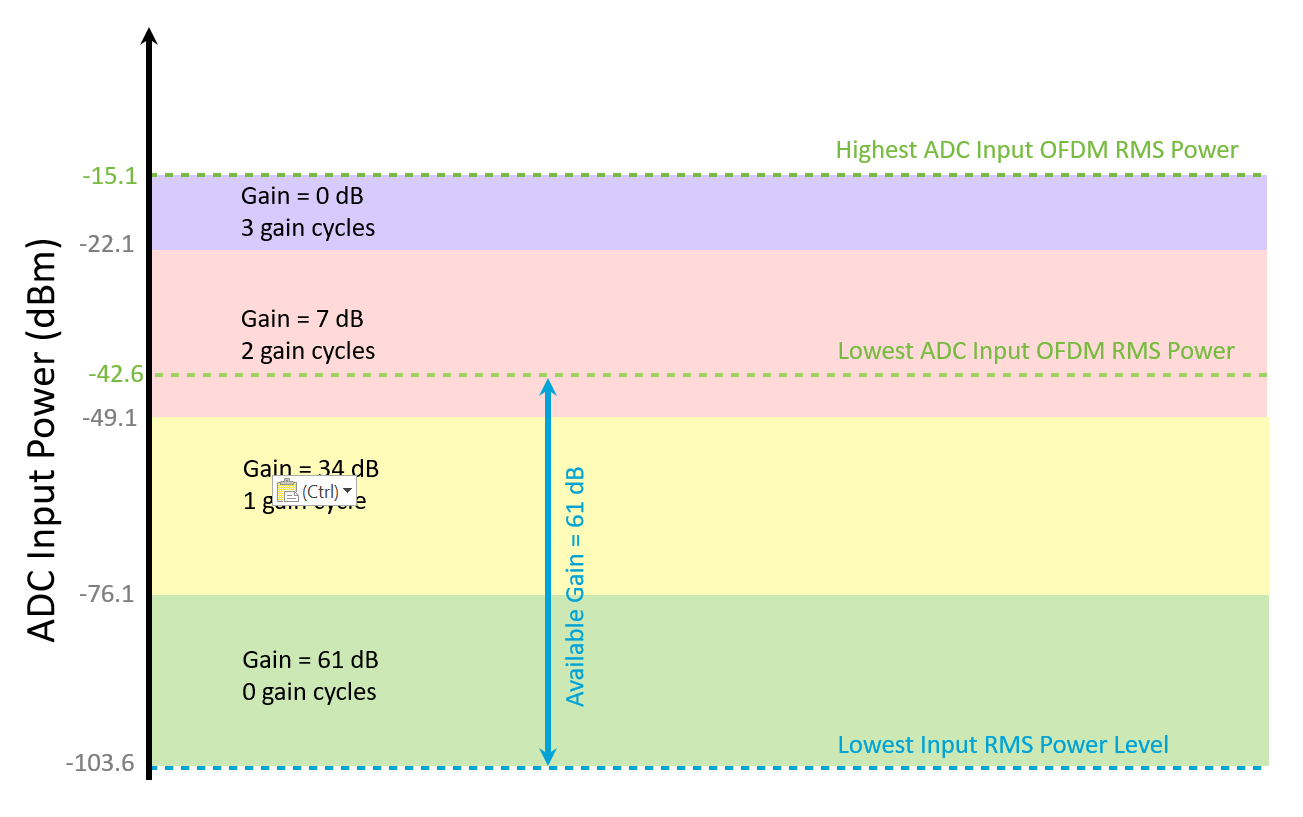
\includegraphics[width=1\linewidth]{./figs/agc/agc_control_ranges}
\caption{AGC input power regions for coarse gain control.}
\label{fig_agc_coarse_gain}
\end{figure}
	
	This entire sequence is governed by a digital Mealy state machine that is triggered upon a packet detection event.
	Implemented with lookup tables in \ac{FPGA} fabric, the AGC state machine flow diagram is given in Figure~\ref{fig_agc_state_machine}.
	Program execution begins once a packet is detected and a issues a trigger signal to bring the machine out of \emph{IDLE} state.
	The state machine then performs successive rounds of saturation detection and removal, entering the fine AGC state once saturation is removed.
	Once the fine gains have been set and a final power estimation round stores the settled input power level for higher layer control, the AGC state machine enters the \emph{IDLE} state, waiting for the next packet detection trigger.
	
	%====================== State Machine Diagram
%http://madebyevan.com/fsm/
\begin{figure}[p]
\begin{center}
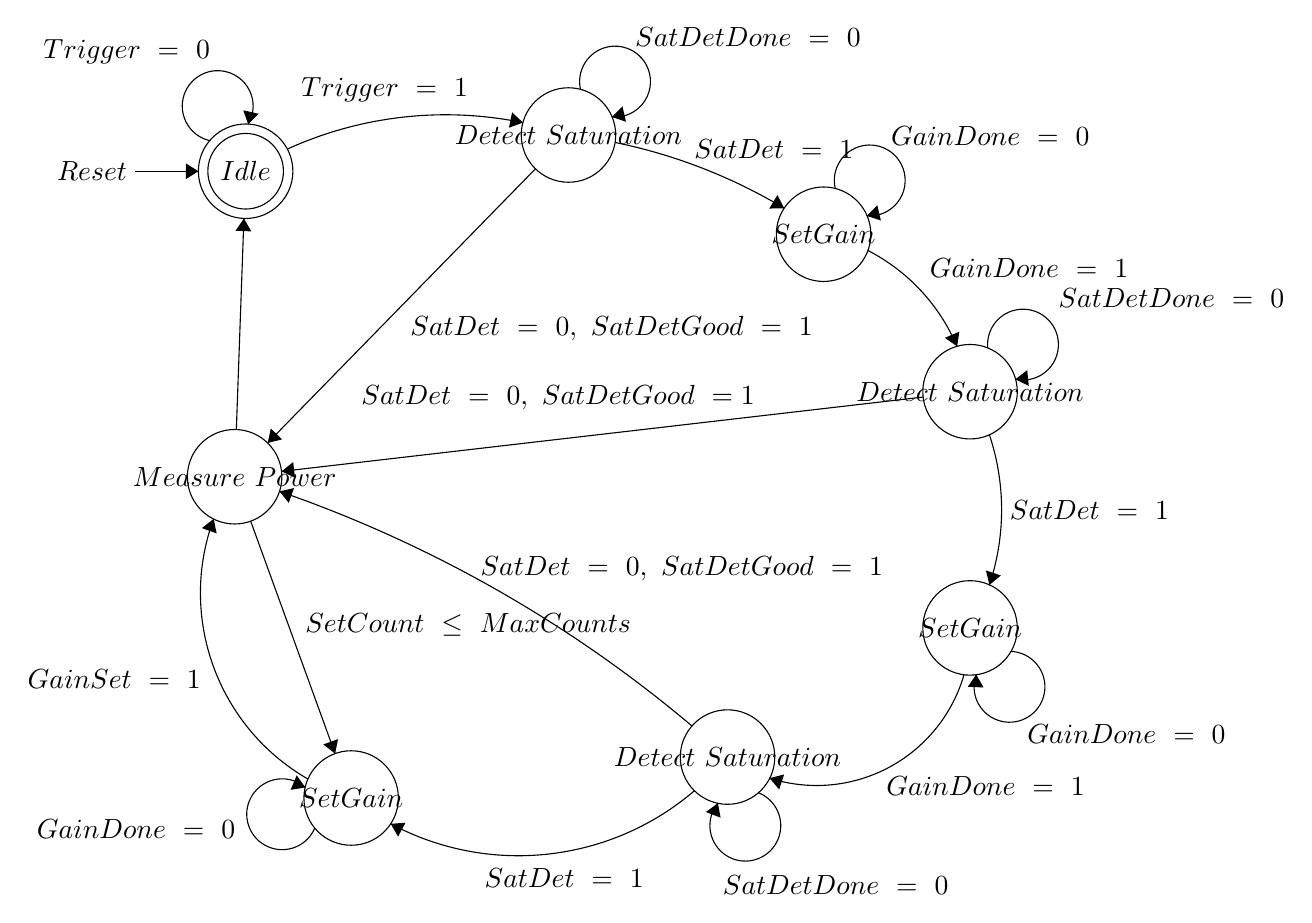
\begin{tikzpicture}[scale=0.2]
\tikzstyle{every node}+=[inner sep=0pt]
\draw [black] (13.7,-10.7) circle (3);
\draw (13.7,-10.7) node {$Idle$};
\draw [black] (13.7,-10.7) circle (2.4);
\draw [black] (34.2,-8.4) circle (3);
\draw (34.2,-8.4) node {$Detect\mbox{ }Saturation$};
\draw [black] (50.4,-14.7) circle (3);
\draw (50.4,-14.7) node {$SetGain$};
\draw [black] (59.7,-24.7) circle (3);
\draw (59.7,-24.7) node {$Detect\mbox{ }Saturation$};
\draw [black] (59.7,-39.7) circle (3);
\draw (59.7,-39.7) node {$SetGain$};
\draw [black] (44.3,-47.9) circle (3);
\draw (44.3,-47.9) node {$Detect\mbox{ }Saturation$};
\draw [black] (20.4,-50.5) circle (3);
\draw (20.4,-50.5) node {$SetGain$};
\draw [black] (13,-30.1) circle (3);
\draw (13,-30.1) node {$Measure\mbox{ }Power$};
\draw [black] (16.347,-9.293) arc (114.45584:78.34724:24.286);
\fill [black] (31.31,-7.61) -- (30.62,-6.96) -- (30.42,-7.94);
\draw (22.53,-6.33) node [above] {$Trigger\mbox{ }=\mbox{ }1$};
\draw [black] (37.161,-8.873) arc (78.41398:59.08501:34.306);
\fill [black] (47.9,-13.05) -- (47.47,-12.21) -- (46.95,-13.07);
\draw (47.24,-9.91) node [above] {$SatDet\mbox{ }=\mbox{ }1$};
\draw [black] (53.209,-15.731) arc (62.82159:23.02406:12.223);
\fill [black] (58.88,-21.82) -- (59.02,-20.89) -- (58.1,-21.28);
\draw (57.11,-16.82) node [right] {$GainDone\mbox{ }=\mbox{ }1$};
\draw [black] (60.928,-27.432) arc (18.48993:-18.48993:15.035);
\fill [black] (60.93,-36.97) -- (61.66,-36.37) -- (60.71,-36.05);
\draw (62.2,-32.2) node [right] {$SatDet\mbox{ }=\mbox{ }1$};
\draw [black] (59.32,-42.664) arc (-16.11491:-107.81738:9.749);
\fill [black] (46.97,-49.24) -- (47.58,-49.96) -- (47.89,-49.01);
\draw (60.68,-49.08) node [below] {$GainDone\mbox{ }=\mbox{ }1$};
\draw [black] (42.201,-50.038) arc (-49.47394:-118.10886:17.209);
\fill [black] (22.91,-52.14) -- (23.38,-52.95) -- (23.85,-52.07);
\draw (33.93,-54.97) node [below] {$SatDet\mbox{ }=\mbox{ }1$};
\draw [black] (17.658,-49.299) arc (-119.96087:-200.16315:13.64);
\fill [black] (11.67,-32.78) -- (10.92,-33.36) -- (11.86,-33.7);
\draw (10.89,-42.92) node [left] {$GainSet\mbox{ }=\mbox{ }1$};
\draw [black] (32.1,-10.55) -- (15.1,-27.95);
\fill [black] (15.1,-27.95) -- (16.01,-27.73) -- (15.3,-27.03);
\draw (24.13,-20.72) node [right] {$SatDet\mbox{ }=\mbox{ }0,\mbox{ }SatDetGood\mbox{ }=\mbox{ }1$};
\draw [black] (56.72,-25.04) -- (15.98,-29.76);
\fill [black] (15.98,-29.76) -- (16.83,-30.16) -- (16.72,-29.17);
\draw (33.54,-25.89) node [above] {$SatDet\mbox{ }=\mbox{ }0,\mbox{ }SatDetGood\mbox{ }=1$};
\draw [black] (15.852,-31.03) arc (70.90436:49.84271:82.428);
\fill [black] (15.85,-31.03) -- (16.44,-31.76) -- (16.77,-30.82);
\draw (41.4,-36.75) node [above] {$SatDet\mbox{ }=\mbox{ }0,\mbox{ }SatDetGood\mbox{ }=\mbox{ }1$};
\draw [black] (14.02,-32.92) -- (19.38,-47.68);
\fill [black] (19.38,-47.68) -- (19.57,-46.76) -- (18.63,-47.1);
\draw (17.46,-39.51) node [right] {$SetCount\mbox{ }\le\mbox{ }MaxCounts$};
\draw [black] (13.11,-27.1) -- (13.59,-13.7);
\fill [black] (13.59,-13.7) -- (13.06,-14.48) -- (14.06,-14.52);
\draw [black] (6.7,-10.7) -- (10.7,-10.7);
\draw (6.2,-10.7) node [left] {$Reset$};
\fill [black] (10.7,-10.7) -- (9.9,-10.2) -- (9.9,-11.2);
\draw [black] (11.428,-8.759) arc (257.22696:-30.77304:2.25);
\draw (6.15,-3.94) node [above] {$Trigger\mbox{ }=\mbox{ }0$};
\fill [black] (13.86,-7.72) -- (14.52,-7.05) -- (13.55,-6.83);
\draw [black] (34.964,-5.511) arc (192.90953:-95.09047:2.25);
\draw (45.6,-2.82) node [above] {$SatDetDone\mbox{ }=\mbox{ }0$};
\fill [black] (36.96,-7.25) -- (37.85,-7.56) -- (37.63,-6.58);
\draw [black] (51.142,-11.805) arc (193.34585:-94.65415:2.25);
\draw (60.98,-9.09) node [above] {$GainDone\mbox{ }=\mbox{ }0$};
\fill [black] (53.15,-13.53) -- (54.04,-13.83) -- (53.81,-12.86);
\draw [black] (62.29,-41.191) arc (87.80455:-200.19545:2.25);
\draw (69.63,-45.81) node [below] {$GainDone\mbox{ }=\mbox{ }0$};
\fill [black] (60.09,-42.66) -- (59.56,-43.44) -- (60.56,-43.48);
\draw [black] (60.824,-21.931) arc (185.63354:-102.36646:2.25);
\draw (65.29,-18.76) node [right] {$SatDetDone\mbox{ }=\mbox{ }0$};
\fill [black] (62.58,-23.91) -- (63.43,-24.33) -- (63.33,-23.33);
\draw [black] (46.253,-50.162) arc (68.53554:-219.46446:2.25);
\draw (51.17,-55.39) node [below] {$SatDetDone\mbox{ }=\mbox{ }0$};
\fill [black] (43.69,-50.83) -- (42.93,-51.39) -- (43.86,-51.75);
\draw [black] (18.094,-52.401) arc (-22.75948:-310.75948:2.25);
\draw (13.07,-52.46) node [left] {$GainDone\mbox{ }=\mbox{ }0$};
\fill [black] (17.49,-49.83) -- (16.94,-49.06) -- (16.56,-49.98);
\end{tikzpicture}
\end{center}
\caption{Mealy state machine diagram of \ac{AGC} operation.}
\label{fig_agc_state_machine}
\end{figure}
	


% Worst-case AGC timing example on WURC platform.
\begin{figure}[p]
\centering
  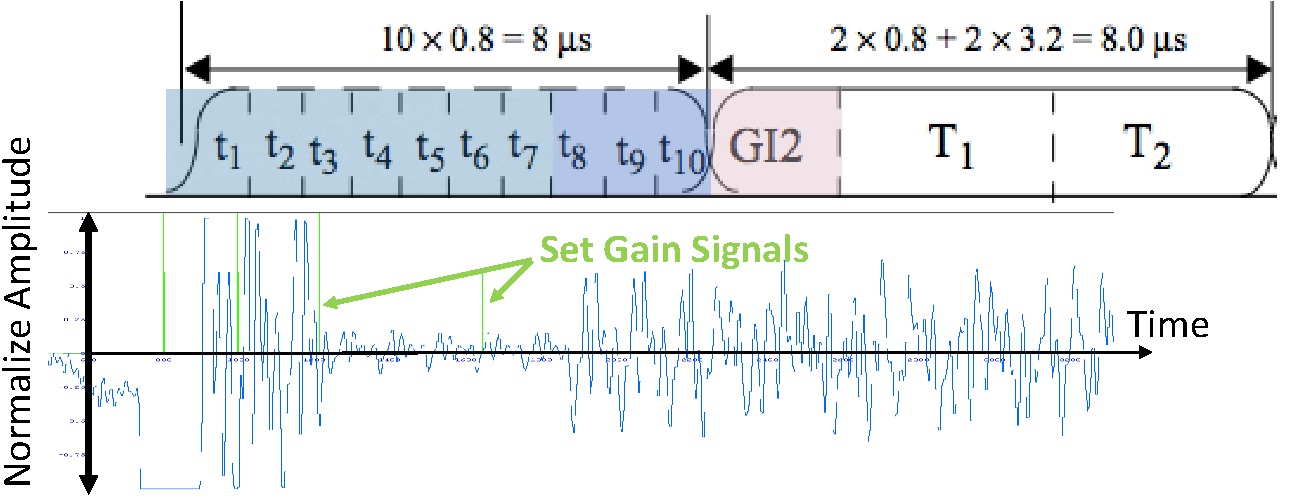
\includegraphics[width=0.9\linewidth]{figs/agc/agc_timing_validation}   
    \caption{Worst-case AGC timing convergence on WURC hardware platform.}
\label{fig_agc_convergence}
\end{figure}
	
\subsection{State Machine Timing Analysis}
\label{sec_agc_timing_analysis}

	In this section, we analyze the timing of the designed system and present recommendations for other system designers to improving timing performance.

	If each saturation detection step take 16 samples and 0.4~$\mu$s at a 40~MHz sampling rate and each round of gain setting takes 0.74~$\mu$s due to the \ac{SPI} bus latency (Section~\ref{sec_agc_timing}), then each coarse gain step takes 1.14~$\mu$s.
	A maximum of three steps takes 3.42~$\mu$s, leaving a remaining 2.18~$\mu$s for packet detection and fine gain control.
	Reliable energy detection of high-SNR signals can be achieved within 16 samples (0.4~$\mu$s), and robust power detection can use any cyclically-shifted version of the 802.11 short training symbols since they are all the same power (0.8~$\mu$s), leaving a small budget of 9 samples (0.225~$\mu$s) for signaling overhead and propagation delays within the digital design.
	
	Unfortunately, in the worst case, when the input signal power is within the purple region in Figure~\ref{fig_agc_coarse_gain}, propagation delay and signaling delays are more than 9 samples, as shown in Figure~\ref{fig_agc_convergence}.
	In this figure, the buffered input \ac{ADC} samples are retrieved from a \ac{WURC} prototype and juxtaposed against the transmitted 802.11 \ac{PLCP} header (top) and the digital gain setting signals (green triggers).
	Three rounds of saturation removal are shown after packet detection (first three green triggers), followed by a long period of fine input power estimation and a final round of gain setting (last green trigger).
	The entire worst-case gain control process is finished within 6.4~$\mu$s, well within the short training preamble, but slightly longer than the 802.11 standards-compliant target of 5.6~$\mu$s.
	
	In each outlined step, decision sample times may be shortened or the logic fine-tuned to reduce the overall worst-case \ac{AGC} convergence time, however it should be clear that the \ac{AGC} timing budget necessitate the use of digital logic as close to the \ac{ADC} as possible.
	
	Luckily, for WARPv3's \ac{OFDM} receiver, the entirety of the 8~$\mu$s short training sequence may be used for \ac{AGC} and fine gain control, thus our system meeting timing requirements for 802.11af-like transmissions utilizing the \ac{WURC} platform.
	Other standards-compliant 802.11 receivers may require that gains must be settled before short training sequence $t_8$, in which case additional optimizations will be required.


%#######################################
\subsubsection{Hardware Controller Architecture}
\label{sec_agc_hw_controller}

	A common design challenge for \ac{SDR} platforms is balancing the desire for flexibility and rapid code development inherent in purely software-based designs with the demand of real-time performance in communications systems.
	We identify a fundamental tradeoff in how the radio physical layer is partitioned: the more abstracted that signal processing becomes from the analog system components, the longer it takes for digital logic to react to events.

\begin{figure}[t] % AGC Design Diagram
\centering
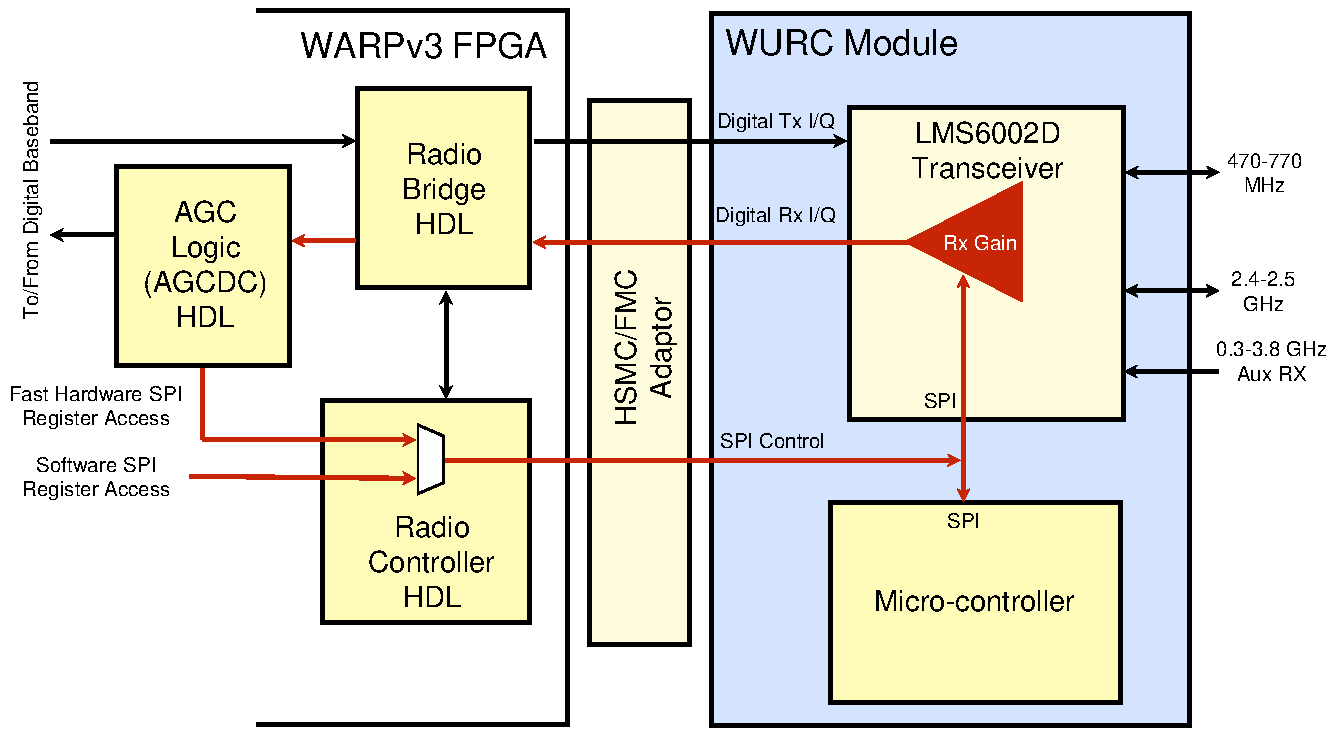
\includegraphics[width=0.9\linewidth]{./figs/agc/agc_block_diagram}
\caption{Hardware control flow of analog AGC design.}
\label{fig_agc_block_diagram}
\end{figure}

	As analog radio transceivers become more integrated and controlled with digital logic, it is important that system designers make architectural decisions that minimize control latencies.
	In order to achieve low-latency operation on \ac{WURC}, we identified time-critical functions such as gain control and embedded their logical functions as close to the digital/analog interface as possible to maximize performance.
	There are four design patterns that are critical to ensuring \ac{SDR} systems can meet high-speed system design demands in \ac{WURC} and other applications:

\begin{enumerate}
\item Direct access to analog control registers from programmable logic or real-time processes enables quick digital reactions,
\item Direct access to analog control registers from software enables cross-layer designs and well-designed software interfaces for complex transceiver configuration options,
\item Register caching in programmable logic avoids lengthy read-modify-write delays when setting analog gains,
\item Control register mappings that consolidate receive gain settings in the smallest number of registers to minimize bus latencies. \label{item_reg_design}
\end{enumerate}

	While we did not have control of Item~\ref{item_reg_design} in this particular system, we observe that transceiver memory maps are increasing in size with complexity and increased programmability and this should be a consideration for future designers of digital transceiver hardware.
	The next-generation LMS7002M utilizes a 16-bit address space with 16-bit depth registers whereas previous generation LMS6002D had an 8-bit address space and 8-bit register depth \cite{lime2012lms6002d, lime2018lms7002M}.
	AD9361 devices use a ``$11+5$'' bit address space and 8-bit register depth.
	However, \ac{SPI} control interfaces remain low-speed for ease of implementation\footnote{\ac{SPI} interface speeds above 50~MHz start to require more advanced design techniques such as length matching, differential signaling, skew and impedance compensation, and provide less safety margin for process variation.}, thus resulting in more time to issue commands to next-generation transceivers.

	The remaining design patterns were implemented with a locally-cached bus arbiter that enabled multi-master direct register access to the LMS6002D transceiver from \textbf{both} high-layer software as well as low-layer programmable logic.
	This new architecture was \emph{required} in order to meet 802.11 standard timing in the \ac{WURC} design without introducing additional analog hardware components as discussed in Section~\ref{sec_agc_related}.
	The multi-master control interface is shown in Figure~\ref{fig_agc_block_diagram}, where both hardware and software \ac{SPI} masters share control over the transceiver \ac{SPI} control bus and arbitration between the masters is implemented in the Radio Controller IP block.
	In addition to performing bus arbitration, the Radio Controller locally caches gain register values so that redundant \ac{SPI} transactions are avoided, eliminating read-modify-write operations in a way that is transparent to the multiple \ac{SPI} masters.
	
	The presented \ac{AGC} logic blocks are available open-source for use in other projects \cite{guerra2012pcores}.
	While some implementation details of this logical design are specific the the hardware platform it was implemented on, the design procedure is generalized for all \acp{SDR} architectures with the same general components as those shown in Figure~\ref{fig_sdr_ideal_rx}.
	In fact, this same system design is being ported to platforms with completely different programmable logic (Xilinx Zynq 7000) and transceiver (Lime Microsystems LMS7002M) subsystems, yet the requirements for high-speed automatic analog gain control have not changed.

%##############################################################3
\subsection{AGC System Evaluation}
\label{sec_agc_system_eval}

	In this section, we evaluate the performance of our fast \ac{AGC} design.
	%Specifically, we are interested in seeing if it can converge fast enough to perform real-time gain control under realistic conditions.
	We wish to show that the designed \ac{AGC} system performs consistently and predictably over all channel gains and consistently meets 802.11 timing requirements.
	A drawback of using the \ac{ADC} as the only sensor for estimating input RF power is that these estimates will be unreliable when the input power falls outside the dynamic range of the \ac{ADC}.
	However, we will show that this system is only unreliable in the high-SNR operating regime where the estimation error does not matter for receiver performance.

\begin{figure}[t]
\centering
  \includegraphics[width=0.9\linewidth]{figs/agc/wsd_manual2_05}   
    \caption{Test setup for AGC evaluation; adjustable attenuator not shown.}
		\label{fig_agc_test_setup}
\end{figure}

	The experimental setup will control the wireless channel between two transmitters to be a simple flat fading channel over a cable between two \ac{WURC} nodes with a variable attenuator (Figure~\ref{fig_agc_test_setup}) where we vary the channel path loss with a variable attenuator in 10~dB steps.
	Assuming that the attenuator provides ideal flat negative gain, this setup ensures that the transmit \ac{SNR} remains constant and the only experimental variables are the receive gain settings and therefore the receive-side \ac{SNR} at the \ac{ADC} input.
	By transmitting a 16-QAM modulated signal (802.11af waveform, 20~MHz channel bandwidth), we are able to detect, decode, and estimate the receive \ac{EVM} of the received signal.
	We expect two sources of increased \ac{EVM}: signals at the \ac{ADC} input that are outside the dynamic range of the \ac{ADC} as identified in Section~\ref{sec_adc_dyn_range}, and decreased \ac{SNR} at the \ac{ADC} input due to weak input power at the antenna port.
	
	With this setup, we program our \ac{AGC} system to target various \ac{ADC} input powers and then transmit 50 802.11af 20~MHz packets constructed in MATLAB using the packet generation framework we built in Section~\ref{sec_static_beamforming}.
		The received packet without \ac{FEC} is decoded and its received \ac{EVM} is calculated as the mean across subcarriers and OFDM symbols of the normalized distance between the received decoded symbol and the intended decoded symbol.

	This experiment is repeated for each target input power between $[-40, 0]$~dBm, with channel attenuation settings between $[60, 100]$~dB in 10~dB steps.
	Figure \ref{fig_agc_rxgain} depicts the performance of the implemented power estimator and \ac{AGC} subsystem design by reporting the mean static receive gain setting that the \ac{AGC} subsystem selected for that packet.
	Error bars in Figure~\ref{fig_agc_rxgain} display the standard deviation across the 50 trials, showing consistent packet detection and input power estimation for all channel attenuation greater than 60~dB.
	At 60~dB, the input power to the \ac{ADC} is so strong that even with all receive gains backed off, the input is still saturated, resulting in inaccurate power estimation and therefore wide variance across selected receive gains for the same input power.
	However, when we look at the receiver \ac{EVM}, we will see that this input gain variance in high input \ac{SNR} conditions is irrelevant to receiver performance.


% AGC RxGain Evaluation
\begin{figure}[ht]
\centering
  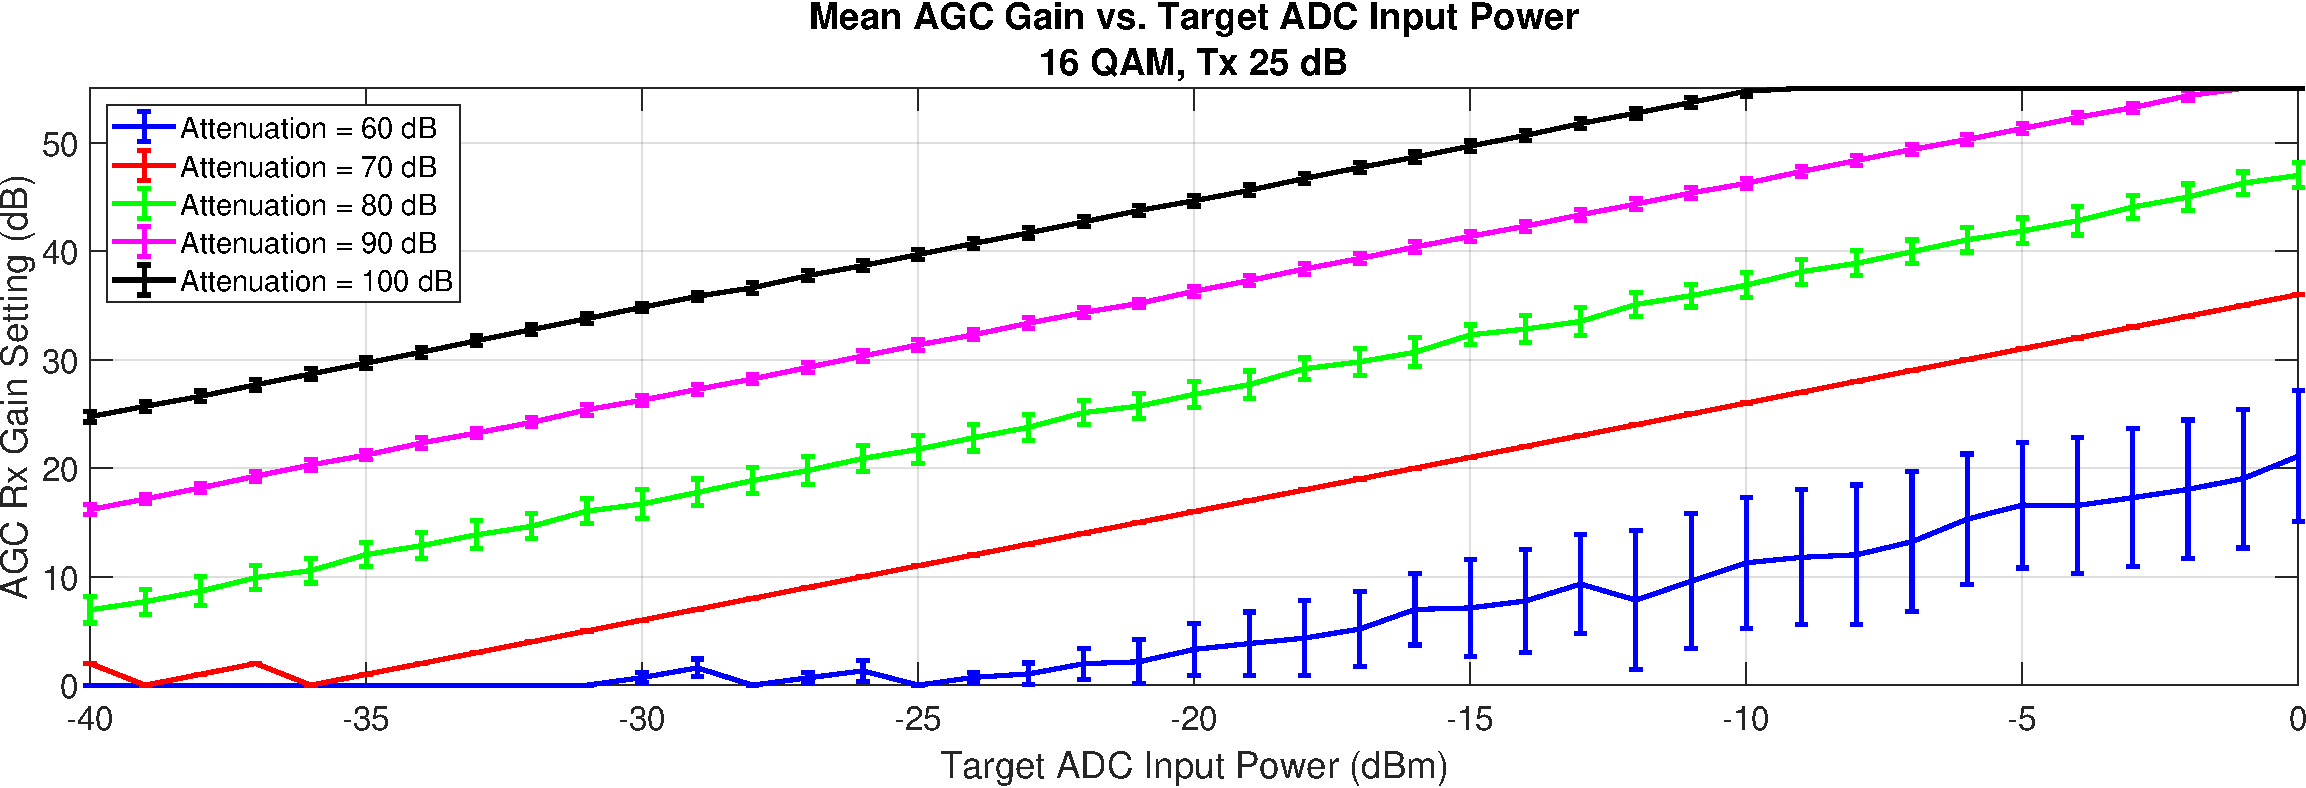
\includegraphics[width=1\linewidth]{figs/agc/AGCTarget_v_EVM_16QAM_ALLdBAtten_Tx25_20MHz_rxgain}   
    \caption{AGC-controlled receive gain setting as a function of ADC input power setting for various channel attenuation and fixed transmit power. Error bars indicate standard deviation across trials.}
\label{fig_agc_rxgain}
\end{figure}
	
	Figure~\ref{fig_agc_evm} shows the measured receive \ac{EVM} for the same set of trials.
	For each attenuation value, the bowl of the EVM curve represents the lower bound on the system's 16-QAM receive EVM, and we have drawn a green shaded region to indicate the target \ac{ADC} input power range that achieves this minimum \ac{EVM} for all input power levels with this 16-QAM modulation.
	The right-most bound of this range is limited by saturation at the ADC and the left-most bound is determined by the system noise floor and quantization error.
	
	% AGC EVM Evaluation
\begin{figure}[hb]
\centering
  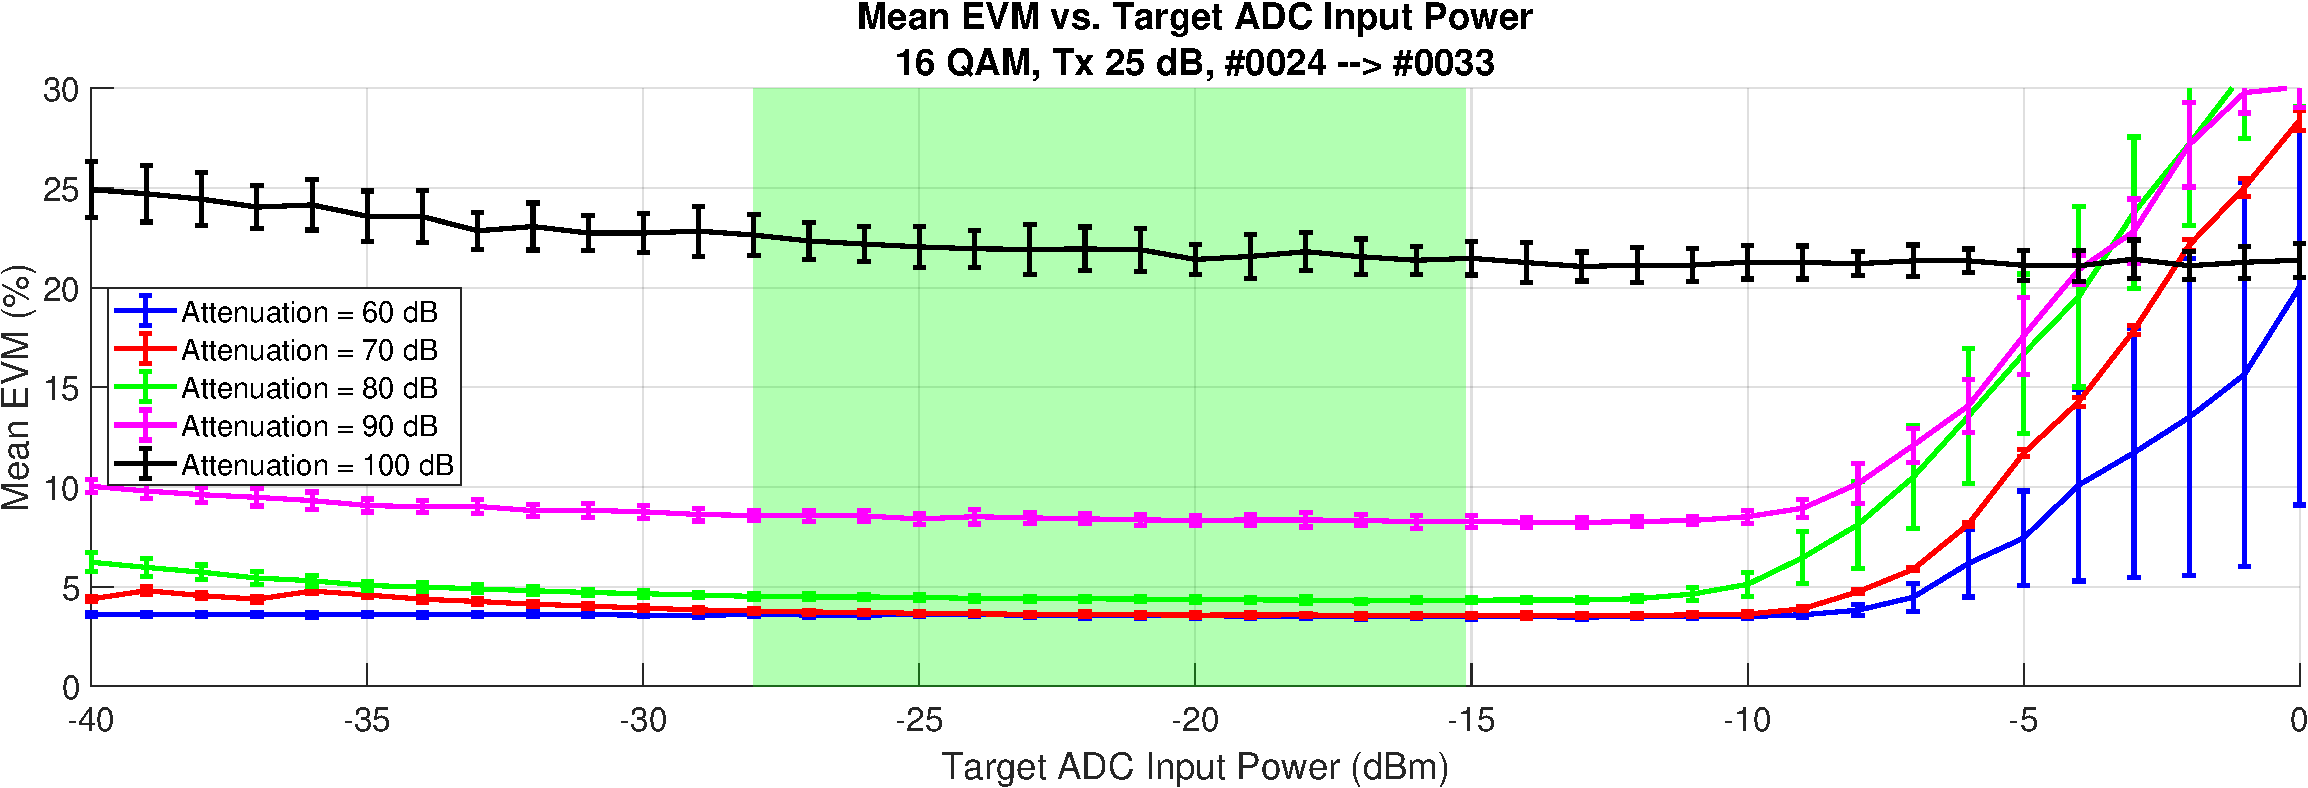
\includegraphics[width=1\linewidth]{figs/agc/AGCTarget_v_EVM_16QAM_ALLdBAtten_Tx25_20MHz_evm}   
    \caption{Received 16-QAM \ac{EVM} as a function of \ac{ADC} input power setting for various channel attenuation. Error bars indicate standard deviation across trials.}
\label{fig_agc_evm}
\end{figure}
	
	To provide some intuition regarding these \ac{EVM} curves, 4\% is the maximum allowed \emph{transmit} \ac{EVM} for an 802.11n transmitter using 64-QAM with $\frac{5}{6}$ coding; 10\% is the maximum allowed transmit \ac{EVM} for 16-QAM with $\frac{5}{6}$ coding; and 2\% is what is required for a 256-QAM transmitter with $\frac{5}{6}$ coding.
	Therefore, although the experiment only used 16-QAM, our implemented system can support the maximum 802.11n modulation rate.
	
	As the channel attenuation increases beyond 70~dB, we see that the achievable minimum \ac{EVM} becomes limited by the signal \ac{SNR} at the \ac{ADC}.
	This effect is particularly obvious at the limits of our testbed at 100~dB channel attenuation, where the mean input power can be reliability estimated as evidenced by the small variance in Figure~\ref{fig_agc_rxgain}, but the receive \ac{SNR} is high and \ac{EVM} becomes dominated by channel and receiver noise in Figure~\ref{fig_agc_evm}.
	
	Based on this evaluation, we fix our target ADC input power to -18 dBm in order to ensure that all received packets are detected and received with minimal quantization error and without clipping.
	This is particular important for the channel measurement studies in Chapter~\ref{sec_environment_chapter}, where channel phase and magnitude estimation accuracy will be important.
	
	Finally, we return to the observation that when the channel attenuation is only 60~dB, saturation causes the \ac{AGC} subsystem to estimate the input signal power inaccurately and select a wide range of receive gain settings for the same input power.
	For the same 60~dB conditions in Figure~\ref{fig_agc_evm}, we can see there is no impact on the \ac{EVM} performance at all in this regime.
	



%##############################################################3
\subsection{Conclusion and Discussion}
\label{sec_agc_conclusion}


	In this section, we have presented the design of an \acf{AGC} system designed for generic \ac{SDR} hardware that does not require the use of external power estimation components.
	We implemented this design on our custom \ac{TVWS} \ac{SDR}, integrating it with the WARPv3 \ac{SDR} platform to construct the first real-time 802.11af-like system with full dynamic range of operation.
	
	A key observation is that the \ac{SPI} control bus between programmable logic and the analog transceiver is the largest arbitrary timing bottleneck, limiting the speed at which we can control receive gains.
	Poor digital design of transceiver register maps has resulted in the need to execute multiple \ac{SPI} bus transactions to change receive gains when fundamentally these settings could be located in a single control register.
	Our recommendation for the design of future \ac{SDR} platforms is to aggregate the digital receiver gain settings in a single control register on the transceiver, making similar \ac{AGC} systems respond more quickly and able to meet even more challenging timing constraints.
	
		While not all \ac{SDR} platforms will be able to use our \ac{AGC} design as-is, we have taken care to present the design motivations and implementation steps such that the same design steps can be applied to other platforms.
	In particular, we discussed the timing limitations required to implement our design in Section~\ref{sec_agc_timing_analysis}; it is clear that \acp{FPGA} or similar programmable digital logic that operates at a high clock speed is required to implement our system and hope to meet very tight 802.11 timing requirements.
	Should another \ac{SDR} platform meet these requirements, then the digital logic blocks we have released open-source \cite{guerra2012pcores} and design procedures we have presented here will allow them to realize the entire dynamic range of their receiver front-end without additional analog hardware components.

